% !TeX root = Report.tex
\section{Implemented Algorithms}

\dirtree{%
.1 Common/.
.2 containers/.
.3 linked-list.[h/c].
.3 array-list.[h/c].
.3 unique-array.[h/c].
.3 map.[h/c].
.2 net/.
.3 eventupdate.[h/c].
.3 multipacket.[h/c].
.3 nhopflood.[h/c].
.3 rimeaddr-helpers.[h/c].
.3 tree-aggregator.[h/c].
.2 debug-helper.[h/c].
.2 led-helper.[h/c].
.2 random-range.[h/c].
.2 sensor-converter.[h/c].
}

\subsection{Container Library}

Contiki comes with a list container \footnote{Header: \url{https://github.com/contiki-os/contiki/blob/master/core/lib/list.h} Source: \url{https://github.com/contiki-os/contiki/blob/master/core/lib/list.c}}, however, when we were developing with their linked list we found that it was awkward to use in some situations (for instance creating an array of lists) so we decided that we needed to find a better list library. Our problem was that other container libraries were unlikely to be optimised to the low memory requirements or support the special compile chain used by Contiki. So rather than waste time searching and integrating an external library we decided to write our own set of containers. By doing the main benefit we gained was that we knew how the containers worked so had a better understanding how to use them.

Another reason to develop our own containers was that we desired an list where the data was stored in an array, this was for because it provides lower memory overhead and the types of operations we would be performing (append and empty) meant that an array backed list would be better. The lower memory overhead comes from the fact that an array-based list doesn't need to store a pointer to the next element as it is implicit (due to the contiguous memory) that a pointer to the current element's pointer plus one is the next element. This means that in a list of $N$ items our singly linked list implementation will require $(\text{sizeof}(T) + \text{sizeof}(void *) \times 2) \times N$ bytes of memory, whereas our array list implementation will require $(\text{sizeof}(T) + \text{sizeof}(void *)) \times N$ bytes of memory.

Our linked list implementation uses more memory compared to Contiki's implementation because their list is \emph{intrusive}\footnote{Boost Containers: \url{http://www.boost.org/doc/libs/1\_53\_0/doc/html/intrusive/presenting\_containers.html}}. What is meant by this is that the pointer to the next item in the list is contained in the structure stored in the list \cite{?}. Meaning their list uses the same amount of memory as our array list. However, because the list is intrusive it makes it more difficult to use as the implementation detail leaks into the structure using the library, this was why developing our own non-intrusive list made it easier to develop code.

We also developed containers that helped abstract certain concepts (such as list uniqueness or accessing elements by key) to decrease code duplication and allow us to express the code in a higher-level way making implementation easier. One thing to note is that for the containers we did not focus on implementing some of their functions to the standard complexity. For example our map implementation has requires O(N) for both insert and fetching, where these may be implemented as O(1) on average (hash tables) or O(log N) (trees), however due to the requirements of low memory we decided to keep using the array as the backing store for the data with the aim to keep memory for at the expense of non-optimal container management functions. The increased time complexity should make little difference as the containers tend to have few elements in them (i.e. hundreds rather than millions, where complexity would start to be important \cite{?}).

Finally, all of these custom containers are tested by a test suite that checks for functional correctness. Also the test suite was run using \verb|valgrind|\footnote{\url{http://valgrind.org/info/tools.html}} to check for memory leaks and corruption.

\subsection{Network Library}

\subsubsection{Event Update}

\subsubsection{Multi-Packet}

In Contiki sending a single packet has its limits, there is only so much data you can get in a single packet. There are two C macros that are relevant to this \verb|PACKETBUF_HDR_SIZE| which is set to 48 bytes and \verb|PACKETBUF_SIZE| which is set to 128 bytes\footnote{packetbuf.h \url{http://contiki.sourceforge.net/docs/2.6/a00302.html}}. This means that in general we will only be able to send a packet containing 128 bytes of information, but what if we have a data structure that spans 300 bytes? Then we will need to have a way to send multiple packets and a receiver that can put the packets back together in the correct way to deliver the data.

Contiki's data transfer primitives for their RIME protocols are fairly hidden because of their focus on uIPv6. We found \verb|ruldolph0| first \footnote{ruldolph0 \url{http://contiki.sourceforge.net/docs/2.6/a01735.html}} and then \verb|rucb| (Reliable Unicast Bulk Transfer) much later \footnote{rucb \url{http://contiki.sourceforge.net/docs/2.6/a00365.html}}. However, both of them have problems, the API is very convoluted and seems more geared towards sending very large files across the network. This is very different to our aim, which is to send relatively small packets of data to a specific neighbour. So we wrote our own API that would split data of any given size and reassemble it once received, our API was not focused on processing data chunks like \verb|ruldolph0| or \verb|rucb|, but simply operated on a block of memory given to it. This is a case where a simpler API made development much easier for us. Admittedly because our implementation uses dynamic memory allocation it could potentially perform worse, but because the energy of sending and receiving messages dwarfs the energy usage of the CPU, we feel that easier development tradeoff made it worth it. Also, now that code has been written to use this API, the \verb|multipacket| library itself could always be rewritten to use \verb|rucb| as a base to run more efficiently.

\subsubsection{N-Hop Request}
We developed the N-Hop Request communication layer early in the project because we needed a way to pass predicate evaluation messages between nodes, these messages needed to be able to travel multiple hops in the network and also contain routing information for the receiver so that they could respond after they've evaluated the predicate. This was a very specific task, unsurprisingly there were no libraries in Contiki suitable for this so instead we developed our own communication layer and API to handle the routing of these messages. 

We used the base level Contiki libraries broadcast, unicast and ctimers. Rime protocol.

The N-Hop Request communication layer was initially heavily influenced by the H-Send\cite{HSEND}.

Node receives a request to evaluate a predicate

\subsubsection{N-Hop Flood}

\subsubsection{Neighbour Detection}

\begin{figure}[ht!]
\centering
\subfigure[Node A requesting neighbour data]{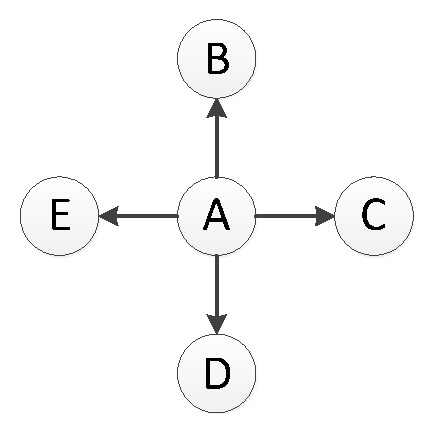
\includegraphics[width=0.25\textwidth]{Diagrams/neighbour-request}}
\subfigure[Node A receiving neighbour data]{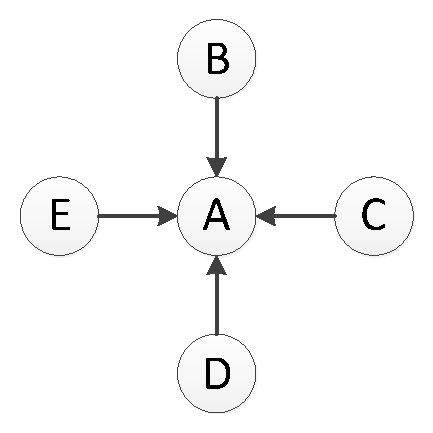
\includegraphics[width=0.25\textwidth]{Diagrams/neighbour-report}}
\end{figure}

\subsubsection{Tree Aggregation}

\begin{figure}[ht!]
\centering
\subfigure[Example Network]{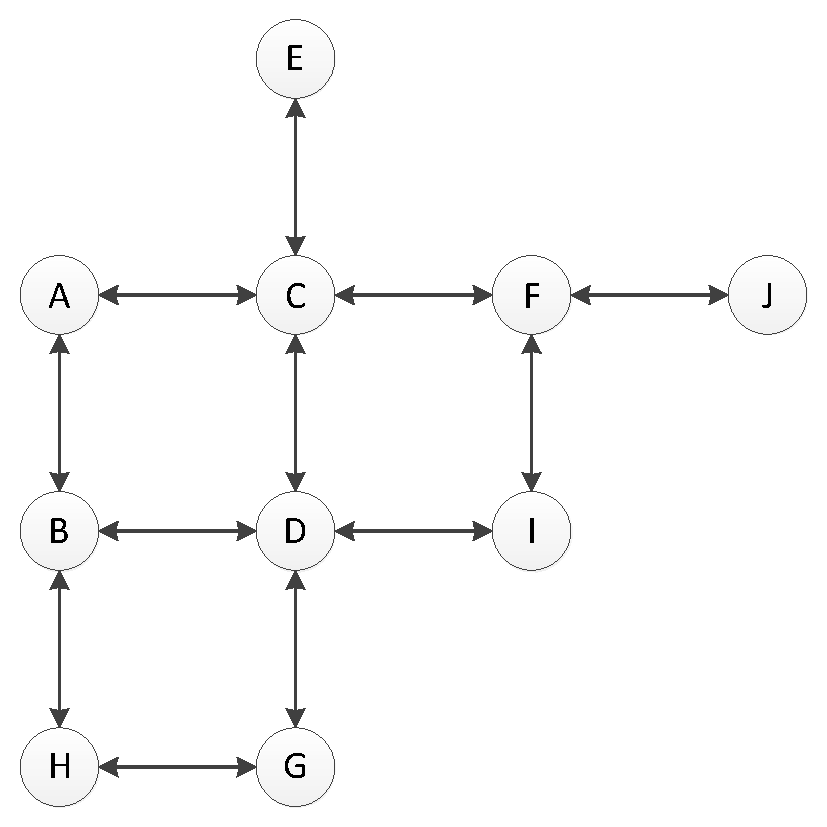
\includegraphics[width=0.75\textwidth]{Diagrams/neighbour-network}}

\subfigure[Logical Tree imposed on network]{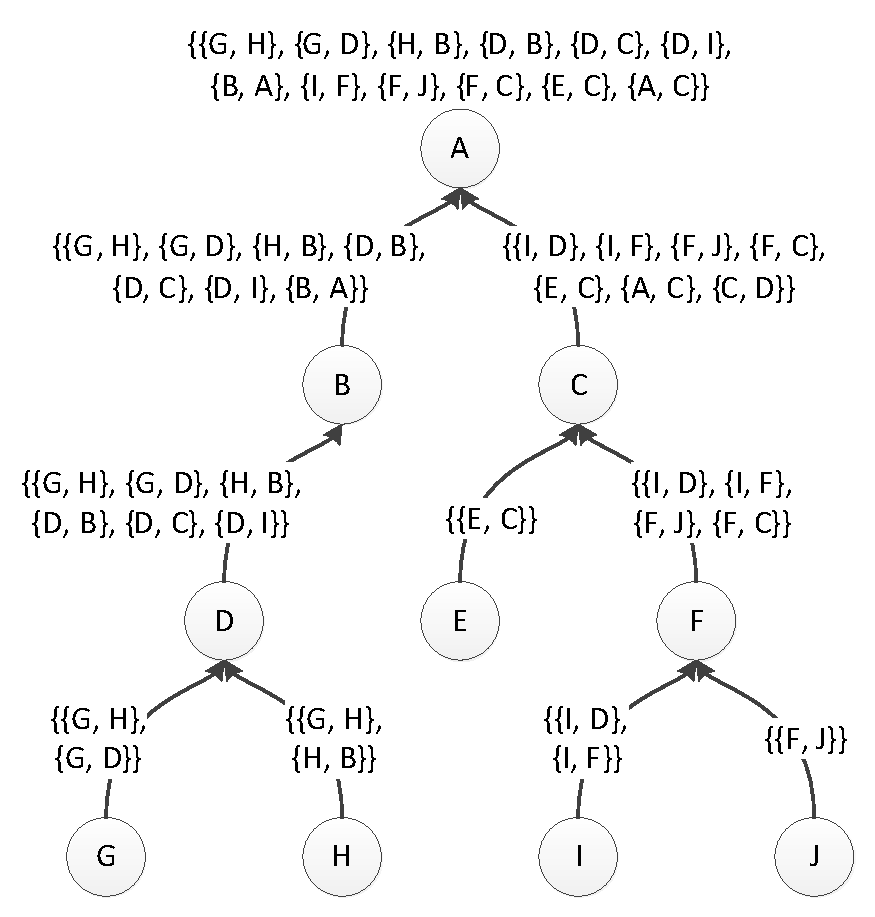
\includegraphics[width=0.75\textwidth]{Diagrams/neighbour-tree-structure}}
\end{figure}

\subsection{Clustering}

\subsection{Hierarchical Clustering}

\subsection{Predicate Evaluation}

\begin{itemize}
	\item[] Began with single hop predicates
	\begin{itemize}
		\item used Mesh to gather information from surrounding nodes, due to implementation, we could only send one message as a one time
	\end{itemize}	
	\item[] Started work on Multi-hop local based predicates
	\begin{itemize}
		\item stubborn broadcast to reliably broadcast to one hop neighbours, who would then rebroadcast the message to their neighbours until the hop limit was reached.
		\item We tried using trickle to return the results back to the originating node. However, due to trickles implementation, only one message could be flooded through the network at one time. 
		\item due to collisions, we used ctimers to delay the responses to messages sent back to the originator node.
		\item next step is to re-implement the algorithm, so that nodes send messages directly back along the chain of nodes they recieved the predicated check message from. This way the messages will be more reliably returned to the orignator node. This also allows for multiple messages to be sent this way.
		\item can't really do it via waiting for nodes to respond - difficult to know how long to wait
		\item[] If each node waits (e.g.) 10 seconds, then messages will be lost as they go backwards, as the originating node will have already sent its message back
	\end{itemize}	
\end{itemize}

\subsection{LEACH}
\cite{LEACH}

